During the initial stages of the project, the goal was that we wanted to develop an autonomous mapping vehicle. We decided that ROS would be the core of our prototype, because at the time, it seemed like the most optimal and most powerful choice for our main operating system. One of the reasons being, is that there is a lot of documentation and resources about ROS, and people had also previously successfully run ROS and created maps using SLAM on a Raspberry Pi~\cite{pibot}\cite{pibotbook}.

\begin{figure}[H]
	\centering
	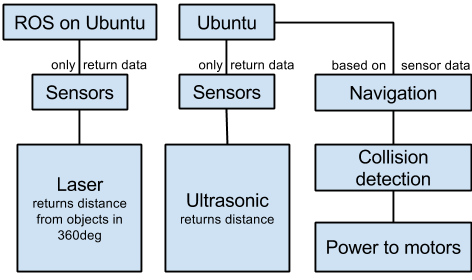
\includegraphics[scale=.7]{images/developmentdiagram2.png}
	\caption{Diagram of the modules we have developed}
	\label{fig:developmentdiagram2}
\end{figure}

Figure \ref{fig:developmentdiagram2} represents the actual implementation of the mapping and navigation system that we built during the development phase of the project. Compared to the initial plans, the \textit{optical flow} sensor was not implemented due not being necessary when using Hector-slam for reference points, as it does its own reference points out of the box. The \textit{remote} module was completely left out of the development, due to the limited time we had to develop it.

Due to an overwhelming time spent on ROS and the laser sensor, we did not manage to create a fully autonomous navigation system, instead we only implemented collision detection, and therefore we decided to split the prototype into two separate parts: 
\begin{itemize}
	\item Navigation system
	\item Mapping system
\end{itemize}

The ROS installation process proved to be quite the challenge, which then lead to a setback in terms of development. Many of the ROS packages caused different conflicts with the Raspbian operating system, even though these packages should have been compatible with the system out of the box. After spending too much time on fixing the many errors and getting it to work on Raspbian, we decided to switch to Ubuntu ARM, where the installation process was much easier compared to the previous one.

For the prototype, we used a CAD design we found on the Internet as a case and rotation platform for the laser. This design was good enough for a prototype, but one of the design-faults we observed was the jittering effect of the gears when rotated by a stepper motor. This forced us to do small step-based calculations using the laser, because it would not take precise microsteps, and therefore our measurements would be off. To overcome this, needed to speed up the rotation. We had separate code for rotating the laser and reading measurements from it, running asynchronously, which made it hard to synchronize the measurements with the rotation , and therefore the maps plotted were too off. We calculated how much time it took to gather readings and tried adjusting the rotation speed accordingly, which in the end turned out to fix our issues, but the speed was too slow compared to our expectations. It took approximately 5 seconds to take a full circle
%TODO: confirm, please
 while gathering readings at every single step the stepper-motor took. Neither the wiringPi or lidarLite libraries, used for communicating with the laser through $I^2C$, were well optimized for the application we wanted to use them in, namely faster data acquisitions. We think this was caused because of a mixture of async- and synchronous code executed in these libraries when writing and reading through the $I^2C$ registry for acquiring new laser data. Also, the laser rotation platform was pretty well thought out, but if our resources would have allowed us, we would have designed our own to fit everything into it and to potentially design better gears.

Hypothetically, if the mapping device would be mounted to the rover, which would be able to navigate areas whilst the mapping device creates a map. However, due to the low-intelligence of the rover, fast speed of movement and the slow rotation and reading of the laser, it would not be able to distinguish unknown places from known places. It would function purely by avoiding an object and thereafter determining an optimal direction away from said object, not navigating based on the map. 

The close proximity detection system, is a low-intelligence autonomous navigation system for the rover. If we succeeded in completing our original scope, the autonomous navigation would have needed to interface with sensors to ensure that it avoided objects at a height that is not recorded by the LIDAR-Lite laser and mapping algorithms. So what we have currently achieved is a navigation system that is able to successfully navigate between obstacles by avoiding them and recalculating its direction according to where it detected the obstacles.

During testing we observed a couple of key-flaws in terms of the close proximity detection systems performance.
As described in the testing chapter, the rover would at times get stuck in corners due to the equality of the measurements recorded by the ultrasonic sensors. Whenever the ultrasonic sensors mounted on either side of the rover would have had their distance threshold exceeded the rover would continuously try to turn to left, hit the one wall of the corner, and then immediately attempt to turn right, hitting the other wall. This can be fixed by changing the code, so that it reverses the rover when the threshold for the side mounted sensors is exceeded. Currently the rover takes three measurements, and then afterwards compares them in the same sequence: \textit{Left -> Right -> Center}. This unfortunately always prioritizes turning left, compared to other choices. Optimally the code should be structured to that the navigation algorithm consists of multiple phases, so that the rover takes measurements in the first phase and before making a directional decision it compares the measurements to each other in the second phase. When the measurements have been compared, the rover then knows what direction would be the optimal to turn towards, in the third phase the measured distance would be compared to a threshold distance, depending on the return from the comparison the rover would then adjust its direction.

Changing the algorithm to something more similar to the one stated above, would add another level of intelligence to the rover, making it more flexible in terms of navigation and decision-making in other situations.

The rover is currently operated by using four DC motors with regular rubber wheels mounted to them. Currently we do not have precise control over how far the rover moves each time it is powered on, although we have encoders mounted on the two front wheels. To increase the accuracy of the distance moved, encoders for the DC motors could have been used to determine the distance travelled. The rover also does not turn consistently each time, which is either an issue with uneven weight distribution on the rover or because of inaccuracy with the signalling. In terms of improving how well the rover turns, the rover needs to be balanced and the amount each wheels turns by cycle needs to be determined. Another possible solution for the turning inconsistency is using tracks for movement instead of four independently operated wheels. Tracks would have a larger guarantee of on-site turning.

Too much time during this project was spent chasing the idea of getting SLAM to work. It was a bad combination of tools, because it seems like that ROS was made for desktop computing and its only recently since embedded systems became powerful enough and compatible to run ROS.
